\documentclass{article}
\usepackage{graphicx} % Required for inserting images
\usepackage{hyperref}
\usepackage{amsfonts}
\usepackage{float}

\title{24.09.03 Light Client and Mithril BLS Signature}
\author{Xun Zhang \quad \quad Wuyun Siqin \quad \quad Bingsheng Zhang \\ 
Zhejiang University, CHN \\
22221024@zju.edu.cn \quad 3210101763@zju.edu.cn \quad bingsheng@zju.edu.cn}

\date{September 3 2024}
\begin{document}

\maketitle

\section{Mithril Light Client}

The basic methodology of our zero-knowledge bridge it to use ZK-SNARK to generate a proof, the target chain can be convinced by verifying the proof.

The ZK-SNARK aims to prove the correctness of a(or a batch of) block header. So the smart contract on the target chain will directly verify the proof, instead of verifying the block header(like a light client).

Thus, the approach of zero-knowledge bridge is to write a circuit of light client process firstly. We need to find out the logic of Mithril(as well as Ouroboros) validating a certificate(or a block header).

\subsection{Mithril Validation Code}

The code is developed by \textbf{Cardano Foundation}, and it's used to communicate with IBC, or \textbf{Cosmos} blockchain. The so-callled \textbf{Cardano IBC Incubator} is a project working towards a bridge implementation to allow exchange of information from a Cardano blockchain to Cosmos SDK based blockchains.\href{https://github.com/cardano-foundation/cardano-ibc-incubator}{[https://github.com/cardano-foundation/cardano-ibc-incubator]}
In the directory './cosmos' , containg all Cosmos SDK related source code including the Cardano light client (or thin client) implementation running on the Cosmos chain. The folder was scaffolded via Ignite CLI with Cosmos SDK 0.50.

We show the Mithril light client code following(actually it is not a light clinet, because Mithril always verify the whole certificate):


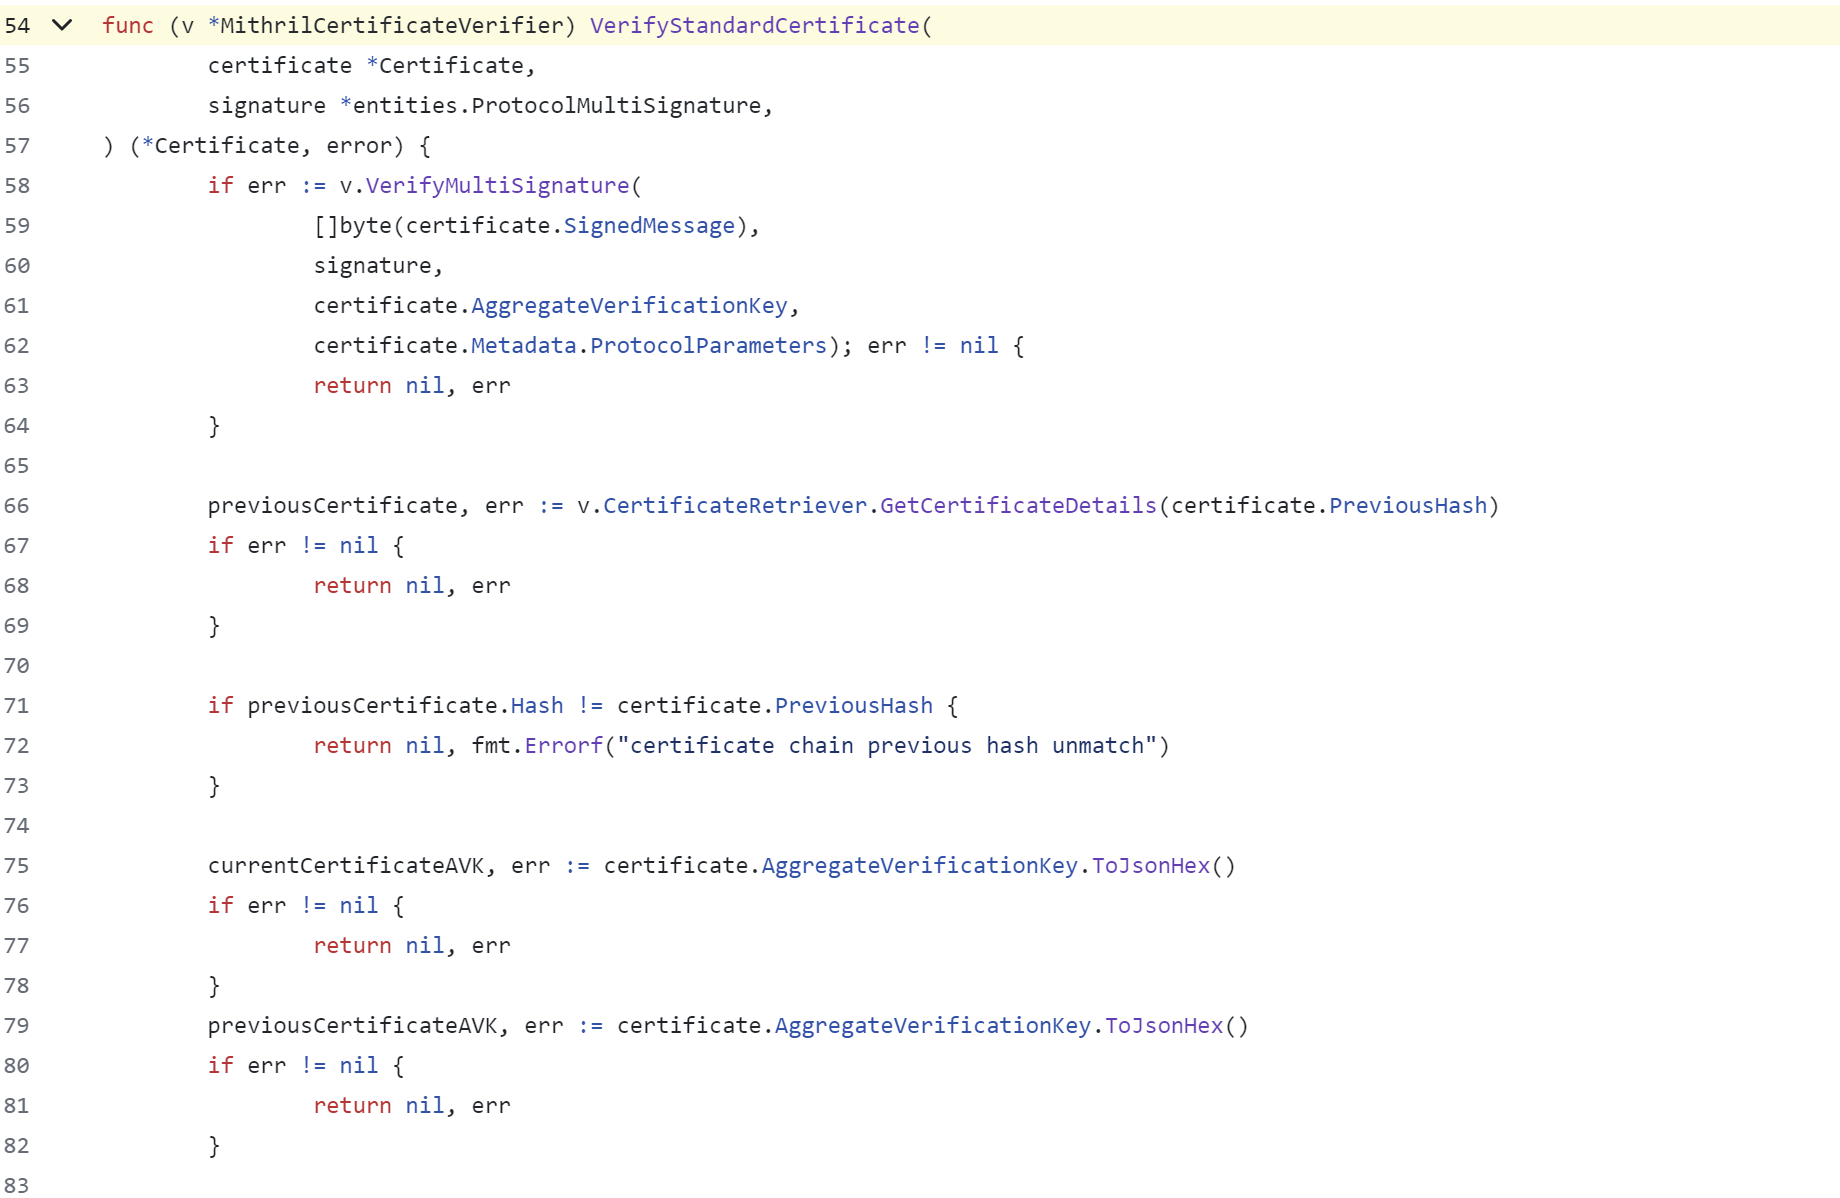
\includegraphics[width=1\linewidth]{cardano-ibc-client-mithril-verifycertificate-1.png}

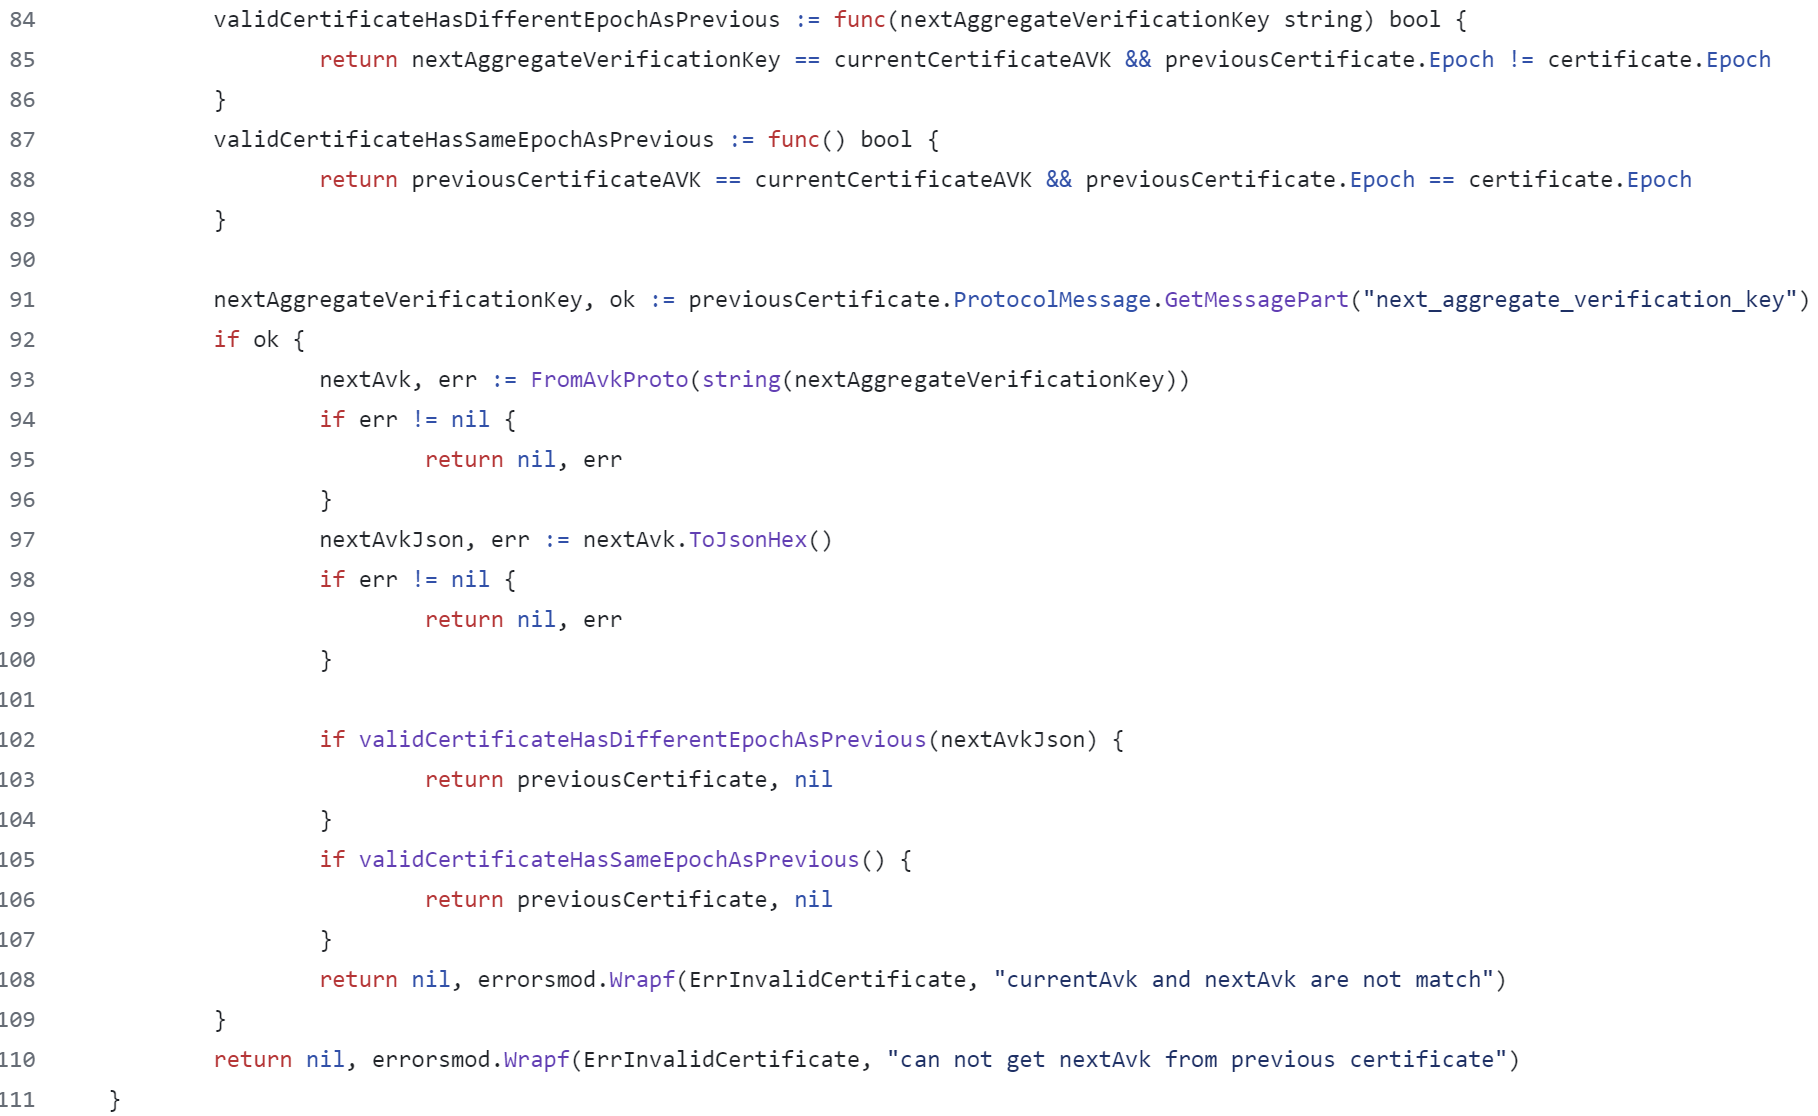
\includegraphics[width=1\linewidth]{cardano-ibc-client-mithril-verifycertificate-2.png}

If we implement the SNARK-based Mithril , then the first check, verifying the multi-signature can be replaced by the \textbf{verifying a halo2 proof}.

So Besides the mulitisignature, there are other checks to do to accept a certificate.

Assuming that we have two certificates, one has been confirmed and stored in memory, and the other one remains to be validated. We call them $\mathsf{previousCertificate}$ and $\mathsf{currentCertificate}$.

So this is a simple scenario of client, because it does not need to validate the genesis certificate, or a chain of certificates, just need to check one "new" certificate.

Following are other checks client need to do:

\begin{enumerate}
    \item check if $\mathsf{previousCertificate.Hash}$ = $\mathsf{certificate.PreviousHash}$ 
    \item if two certificates in same epoch:
        \begin{itemize}
            \item $\mathsf{previousCertificateAVK = currentCertificateAVK}$
            \item $\mathsf{previousCertificate.Epoch = certificate.Epoch}$
        \end{itemize}
    \item if two certificates in different epoch:
        \begin{itemize}
            \item $\mathsf{previousCertificate.next\_aggregate\_verification\_key = currentCertificateAVK}$
            \item $\mathsf{previousCertificate.Epoch != certificate.Epoch}$
        \end{itemize}
\end{enumerate}


\subsection{Cardano Validation Code}

The validation logic is very complex in original code, we extract some important parts of code to see, how we verify a cardano block data in Cosmos chain.

There is a concept names "client state" in this code. Briefly speaking, a client state stores the information of a cardano light client, and the light client uses it to check the new block, and then updates its "client state"(if pass).

The following code shows how a client verifying a block's data:
\\
\\


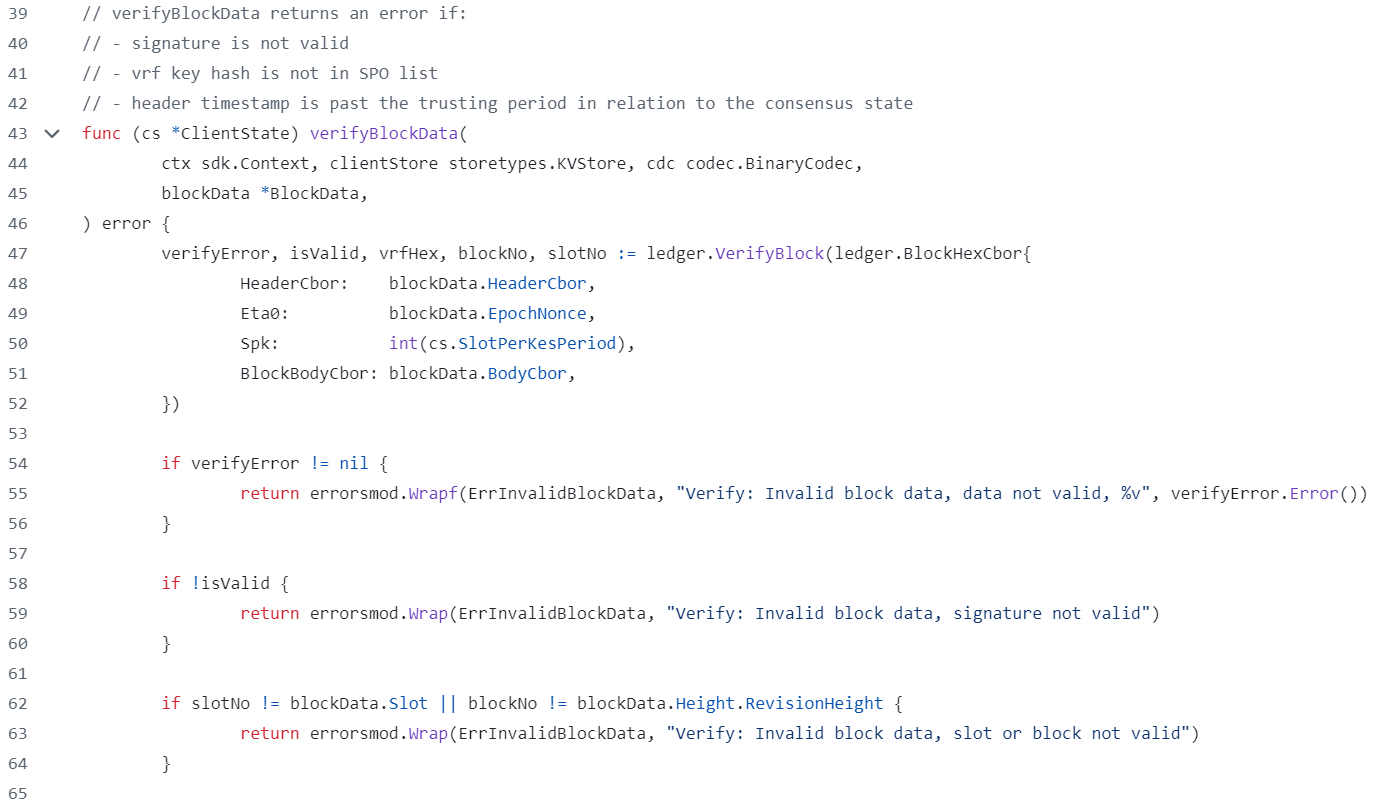
\includegraphics[width=1\linewidth]{cardano-ibc-client-cardano-update-verifyblockdata-1.png}

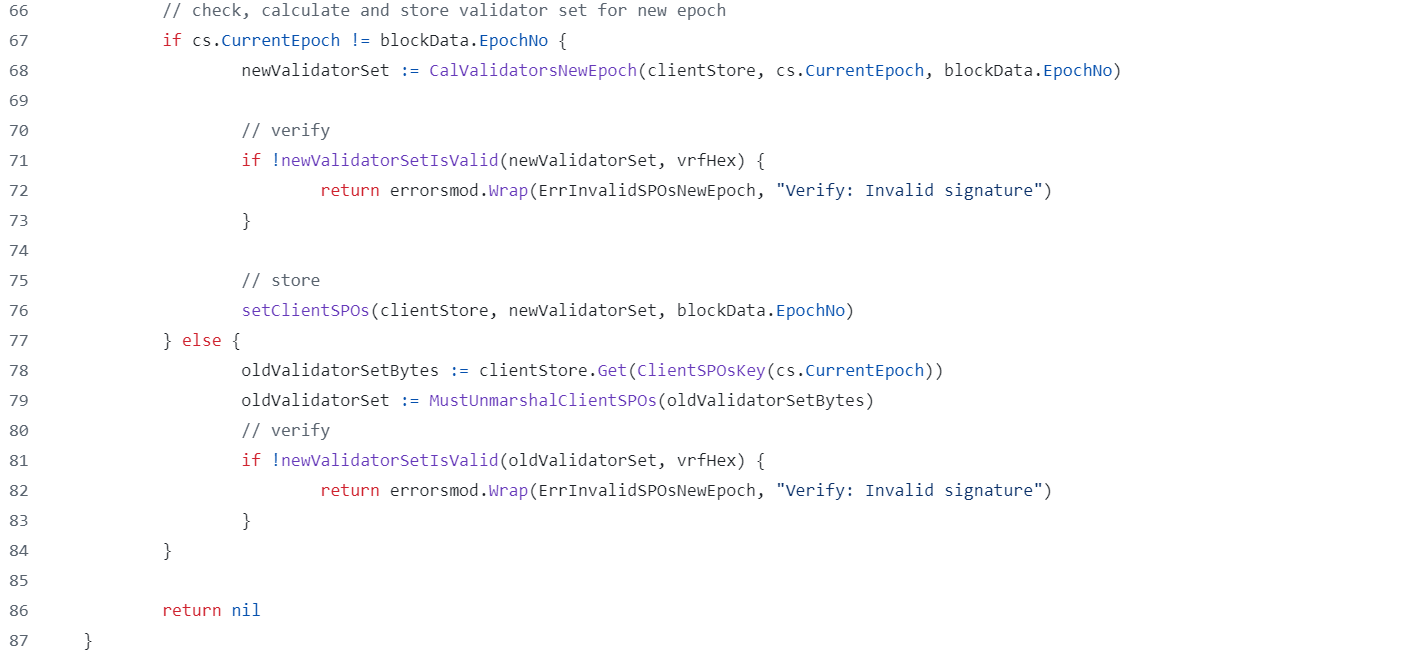
\includegraphics[width=1\linewidth]{cardano-ibc-client-cardano-update-verifyblockdata-2.png}
\\
\\
This code uses methods in other files, so we just simply introduce what have been done in the checking process. The detailed explanation is coming soon.


\begin{itemize}
    \item VerifyBlock function:
        \begin{enumerate}
            \item Check is KES valid.
            \item Check is VRF valid.
            \item Check if block data valid.
        \end{enumerate}
    \item Check slot and height.
    \item Check if it is a new epoch:
        \begin{enumerate}
            \item Yes. Verify the signature of new validators set and store.
            \item No. Verify the signature of old validators set.
        \end{enumerate}
\end{itemize}

Above is the rough logic of a Cardano light client.


\section{Mithril BLS Signature and Benchmark}

In Mithril paper, the pairing check of BLS signature is like following:
\\
\\
$\mathsf{MSP.Ver}(msg, mvk, \sigma)$:Return 1 if $ e(\sigma, g2) = e(\textrm{H}_{\mathbb{G}_1}
(''M''||msg), mvk).$ Otherwise return 0.
\\
\\
But in halo2-lib code, the signature $\sigma$ and message hash is in $\mathbb{G}_2$ and the verification key is in $\mathbb{G}_1$.

So we modify the code of BLS signature verification and benchmark it.
Following are our new results.


\begin{table}[H]
    \centering
    \begin{tabular}{p{1cm}|p{1cm}|p{1cm}|p{2cm}|p{1.5cm}|p{1.5cm}|p{1.5cm}|p{1.5cm}} \hline
          degree&advice&lookup&lookup\_bits&limb\_bits&proof\_time&proof\_size&verify\_time \\ \hline
14&	211&27&		13&	91&		34.5397s&	95808&	42.6186ms\\ \hline
15&	105&14&		14&	90&		31.7353s&	48000&	25.6577ms\\ \hline
16&	50&	6&		15&	90&		26.1168s&	22752&	19.5484ms\\ \hline
17&	25&	3&		16&	88&		24.6446s&	11520&	12.2392ms\\ \hline
18&	13&	2&		17&	88&		25.1638s&	6080&	10.6350ms\\ \hline
19&	6&	1&		18&	90&		25.0424&	3072&	7.4521ms\\ \hline
20&	3&	1&		19&	88&		35.0907s&	1920&	12.2006ms\\ \hline
21&	2&	1&  	20&	88&		54.0728s&	1344&	5.5069ms\\ \hline
22&	1&	1&		21&	88&		89.5040s&	960&	10.0790ms\\ \hline
      
    \end{tabular}
    \caption{Bn254 BLS Signature($\sigma$ on $\mathbb{G}_1$)}
    \label{tab:my_label}
\end{table}

Compare to the original BLS signature(built in halo2-lib code), the Mithril BLS signature is slower(\textasciitilde15s vs \textasciitilde25s)


\subsection{Combine New BLS Signature with Merkle Tree}

In the previous code, we use Poseidon hash function as the building block of merkle tree, the rate of Poseidon is set to 2.
Thus we use a \textbf{ZERO} padding. But since we switch to a verification key in $\mathbb{G}_2$, it is natural use a $\mathbb{G}_2$ element as a hash input, because two 'coefficients' of $\mathbb{G}_2$ element is in  $\mathbb{F}_p$:

\[
\textrm{Original: Poseidon.input = $[pk.x, F:ZERO]$}
\]
\[
\textrm{New: Poseidon.input = $[pk.x.c0, pk.x.c1]$}
\]
\\


However, in our development schedule, we should add the signer's stake(or the $\phi$ evaluation of stake as a optimization), so the rate of Poseidon will be 3, and the construction will be:

\[
\textrm{Plan: Poseidon.input = $[pk.x.c0, pk.x.c1, \phi(\mathsf{stake_i})]$}
\]
\[
\textrm{Plan: Merkle\_Path.input = $[\mathsf{leaf}, \mathsf{path_i}, F:ZERO]$}
\]
\\


\end{document}
